\chapter{Sezioni}

\begin{figure}[H]
 \centering
 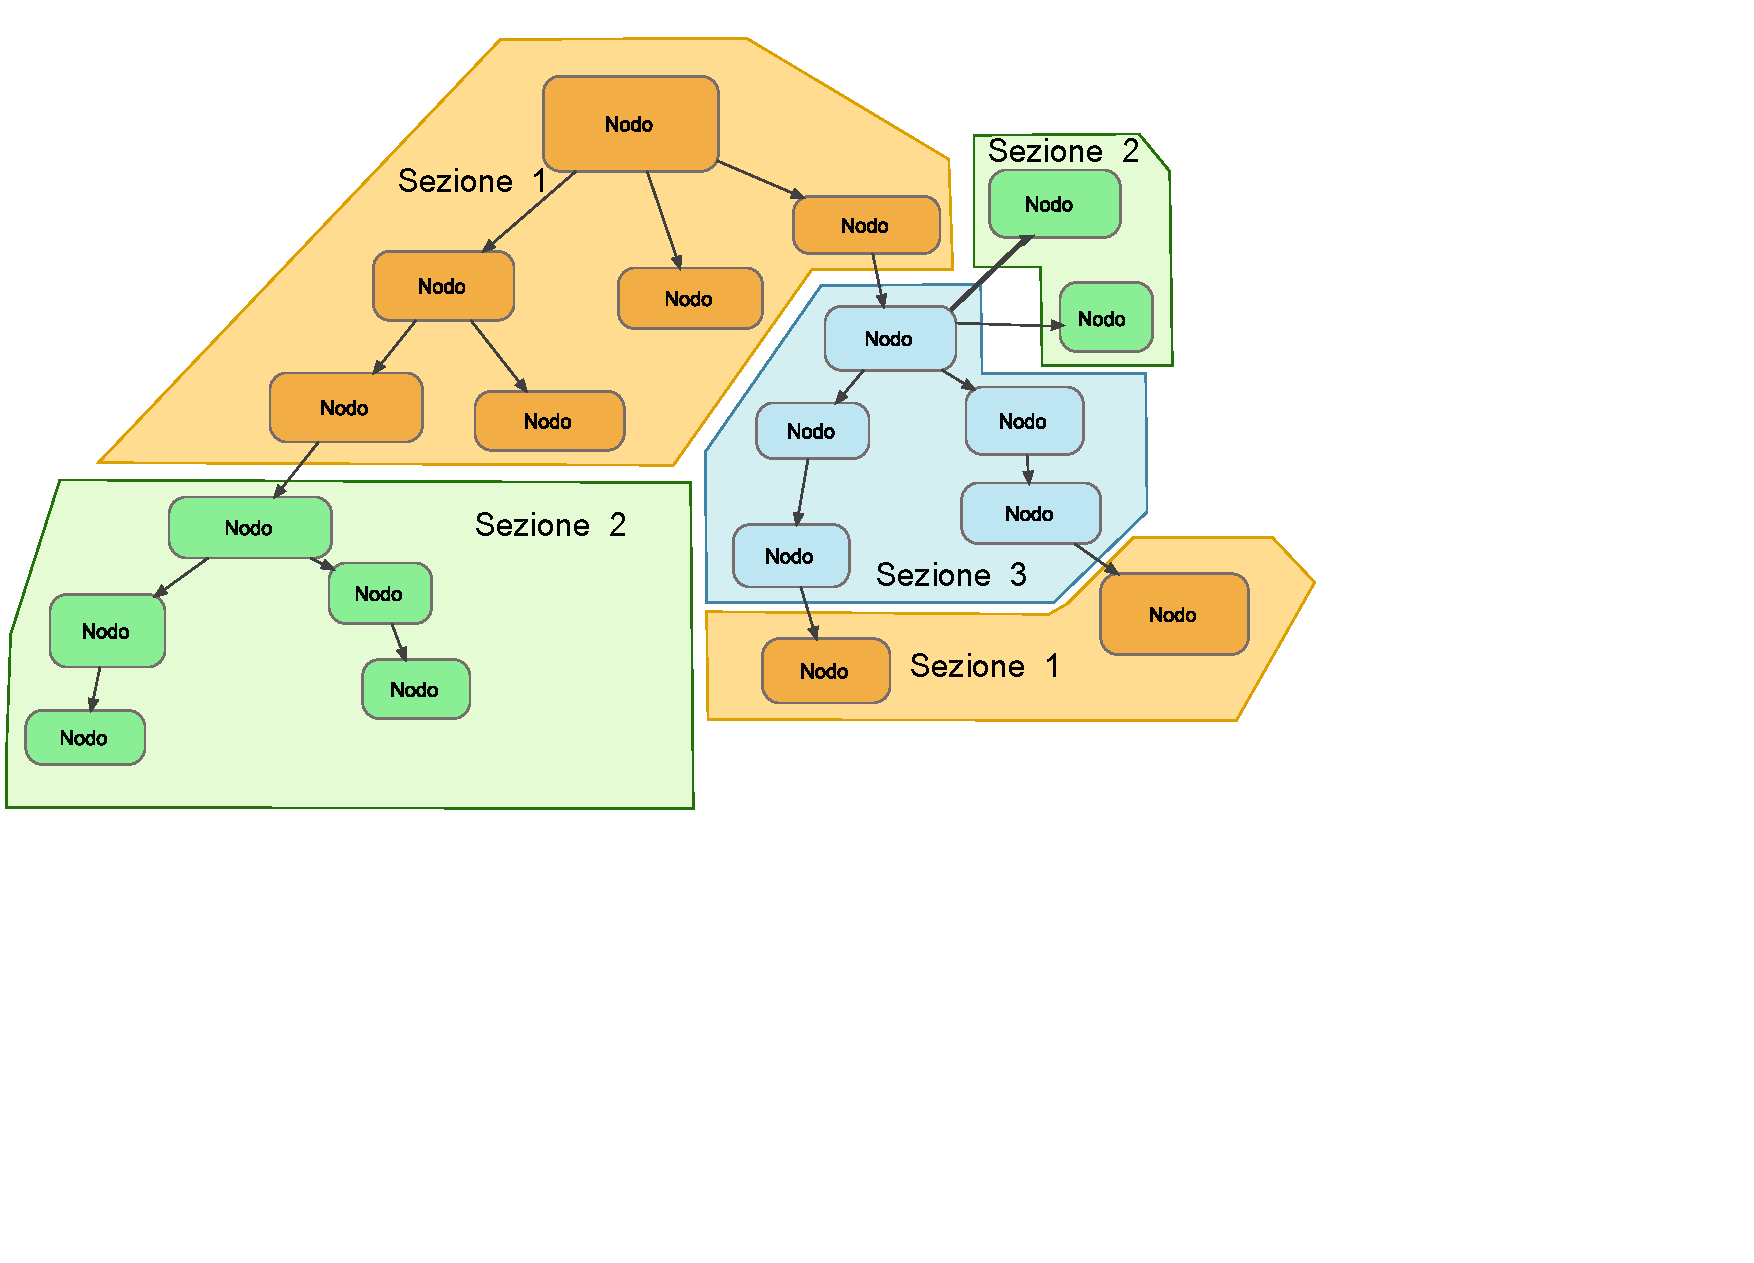
\includegraphics[width=\textwidth]{./immagini/sezioni/sezioni.png}
 % sezioni.pdf: 595x842 pixel, 72dpi, 20.99x29.70 cm, bb=
 \label{fig:sez_schema}
\end{figure}


Le sezioni sono delle etichette che è possibile associare ai contenuti e che ci permettono di creare collezioni virtuali di nodi. Tramite tali etichette possiamo ad esempio:
\begin{itemize}
 \item Segmentare i contenuti del sito in sottoalberi
 \item Cambiare il tema grafico del sito di sezione in sezione
 \item Limitare l'accesso ad alcune aree del sito
 \item Specificare contenuti soggetti all'approvazione da parte di altri utenti
\end{itemize}
\section{Proprietà delle sezioni}
Un ID di sezione  è un numero identificativo che può essere associato ad un oggetto per donotare la sezione a cui questo appartiene. L'ID è memorizzato in un attributo speciale dell'oggetto e non è visibile nell'interfacci di modifica del contenuto. Una sezione può essere assegnata a più oggetti ma un oggetto \emph{può avere un'unica sezione}.
L'assegnazione di differenti ID di sezione a diversi oggetti ci permette di creare una gerarchia logica in parallelo alla struttura ad albero dei contenuti.
Ad ogni ID di sezione è assegnato un nome ad esempio \textsl{Standard} o \textsl{Restricted} e un indicatore di navigazione ad esempio \textsl{Struttura contenuti} o \textsl{Media}. Il nome viene utilizzato per una immediata identificazione della sezione nell'interfaccia di amministrazione, l'indicatore di navigazione  determina invece in quale tab amministrativa verremo posizionati quando accediamo all'oggetto.

\section{Ereditarietà delle sezioni}
  
Quando un oggetto viene creato, ma non è ancora stato pubblicato e quindi è ancora nello stato di bozza, la sua sezione è \textsl{Sezione standard}. Quando l'oggetto è in stato di bozza è accessibile unicamente all'utente che lo ha creato, la sezione assegnatagli è quindi, in questo momento, ininfluente.
Nel momento della pubblicazione dell'oggetto, quando cliccate su \emph{Pubblica}, questo eredita la sezione del suo nodo padre. Ad esempio se create un nuovo oggetto come figlio di un Folder appartenente alla sezione \textsl{Restricted} questo apparterrà a sua volta a tale sezione.

\section{Creazione di una sezione}

Vediamo ora come creare una nuova sezione. Vogliamo prepare un'area riservata per i docenti andremo quindi a preparare una sezione che chiameremo \textsl{riservata\_docenti}
Per prima cosa clicchiamo sulla Tab Impostazioni e poi dal menu sulla sinitra Sezioni:

\begin{figure}[H]
 \centering
 \includegraphics[width=\textwidth]{./immagini/sezioni/interfaccia_sezioni.png}
 % interfaccia _sezioni.png: 926x421 pixel, 72dpi, 32.67x14.85 cm, bb=
 \caption{Interfaccia per la gestione delle sezioni}
 \label{fig:sez-interfacciadocenti}
\end{figure}

una volta avuto accesso all'interfaccia di gestione delle sezioni clicchiamo sul tasto \textsl{Nuova sezione} in modo da accedere all'interfaccia di creazione:
\begin{figure}[H]
 \centering
 \includegraphics[width=\textwidth]{./immagini/sezioni/creazione_sezione.png}
 % creazione_sezione.png: 927x226 pixel, 72dpi, 32.70x7.97 cm, bb=
 \caption{Interfaccia per la creazione di una sezione}
 \label{fig:sez_interfaccia_crea}
\end{figure}
La nostra nuova sezione è ora pronta dobbiamo solo modificare il ruolo assegnato agli insegnanti in modo da dar loro la possibilità di accedere a contenuti appartenenti a questa sezione.
Per questo agiamo come spiegato nel capitolo sui permessi. Andiamo su \textsl{Account utenti} quindi su \textsl{Ruoli e polize} selezioniamo il Ruolo \textsl{Prof editor} e modifichiamolo:
\begin{figure}[H]
 \centering
 \includegraphics[width=\textwidth]{./immagini/sezioni/sezione_ruoli.png}
 % sezione_ruoli.png: 929x428 pixel, 72dpi, 32.77x15.10 cm, bb=
 \caption{Modifica del ruolo assegnato agli insegnanti}
 \label{fig:sez_modifica_ruolo}
\end{figure}

Inseriamo una nuova Poliza di lettura in questo ruolo clicchiamo su \textsl{Nuova policy} e dalla prima schermata della procedura guidata per l'inserimento della poliza scegliamo il modulo \textsl{Content}:

\begin{figure}[H]
 \centering
 \includegraphics[width=\textwidth]{./immagini/sezioni/sezione_ruoli2.png}
 % sezione_ruoli2.png: 934x399 pixel, 72dpi, 32.95x14.08 cm, bb=
 \caption{Creazione di una nuova Poliza nel ruolo Prof editor: scelta del modulo}
 \label{fig:sez_modificaruolo2}
\end{figure}

dopo aver scelto il modulo la procedura guidata ci chiede a quale funzione vogliamo dare accesso, scegliamo \textsl{Read} e clicchiamo su \textsl{Assegna con limitazione}:
\begin{figure}[H]
 \centering
 \includegraphics[width=\textwidth]{./immagini/sezioni/sezione_ruoli3.png}
 % sezione_ruoli3.png: 933x570 pixel, 72dpi, 32.91x20.11 cm, bb=
 \caption{Scelta della funzione a cui dare accesso}
 \label{fig:sez_sezioneruolo3}
\end{figure}

come ultima cosa scegliamo le limitazioni, in questo caso dovremo scegliere nella casella delle sezioni quella appena creata: \textsl{riservata\_docenti}:
\begin{figure}[H]
 \centering
 \includegraphics[width=\textwidth]{./immagini/sezioni/sezione_ruoli4.png}
 % sezione_ruoli4.png: 926x259 pixel, 72dpi, 32.67x9.14 cm, bb=
 \caption{Selezione della sezione a cui far accedere i docenti in lettura}
 \label{fig:sez_modifcaruolo5}
\end{figure}

salviamo ora il nuovo ruolo e prepariamo ad assegnare la sezione agli oggetti che dovranno appartenere all'area riservata. 
Immaginiamo che sia stato precedentemente creato un Folder all'interno del nodo principale del sito, chiameremo questo Folder \emph{Area riservata}. Ritorniamo nell'interfaccia di gestione delle sezioni, individuiamo la sezione precedentemente creata (attenzione potreste dover utilizzare il link \textsl{Successivo} per accedervi).
\begin{figure}[H]
 \centering
 \includegraphics[width=\textwidth]{./immagini/sezioni/sezione_assegna.png}
 % sezione_assegna.png: 930x28 pixel, 72dpi, 32.81x0.99 cm, bb=
 \caption{Assegnamento della sezione ad un oggetto}
 \label{fig:sez_assegna}
\end{figure}

Dobbiamo cliccare sul tasto aggiungi come in figura.\ref{fig:sez_assegna} verranno visualizzati tutti i contenuti del sito per permetterci di selezionare il Folder \textsl{Area riservata}:
\begin{figure}[H]
 \centering
 \includegraphics[width=\textwidth]{./immagini/sezioni/sezione_assegna2.png}
 % sezione_assegna2.png: 950x371 pixel, 72dpi, 33.51x13.09 cm, bb=
 \caption{Selezione del oggetto cui assegnare la sezione}
 \label{fig:sez_asegna2}
\end{figure}

selezioniamo il Folder di interesse a clicchiamo su seleziona. Da ora in poi tale cartella apparterrà alla sezione riservata e vi apparterranno anche tutti i contenuti creati d'ora in poi.
Se visualiziamo il Folder  in \textsl{Struttura contenuti} notiamo che la sua sezione è ora \textsl{riservata\_docenti}:
\begin{figure}[H]
 \centering
 \includegraphics[width=\textwidth]{./immagini/sezioni/sezione_assegnata.png}
 % sezione_assegnata.png: 946x42 pixel, 72dpi, 33.37x1.48 cm, bb=
 \caption{La sezione è stata assegnata al contenuto}
 \label{fig:sez_assegnata}
\end{figure}















